\documentclass[12pt,a4paper]{article}
\usepackage{ssn-be-cse-review}
\usepackage{float}
\usepackage{url}
\usepackage{alltt}
\usepackage{longtable}
%\usepackage{mathtools}
\usepackage{algorithm2e}[1]
\usepackage{tikz}
\usetikzlibrary{shapes,arrows}
\usetikzlibrary{trees}


\begin{document}
   
\ptitle{Project Title}
\review{1}
\setnauthors{4}
\setauthorone{N Kalaichelvi}{312212405011}
\setauthortwo{N Kalaichelvi}{312212405011}
\setauthorthree{N Kalaichelvi}{312212405011}
\setauthorfour{N Kalaichelvi}{312212405011}
\semester{7}
\guide{Sheerazuddin}
\reviewdate{28 August 2013}

\reviewtitle
\hrule

\section{Motivation}
Normal Information Extraction (IE) Systems extract only explicitly
stated information from natural language text. These systems do not
have access to commonsense knowledge, and hence incapable of
performing deeper inference. To identify the facts which are implicit,
commonsense knowledge is needed. A statistical relational learning
approach, namely Bayesian Logic Programs (BLPs) that combines
first-order logic and Bayesian networks, is suitable to infer
additional implicit information.

\section{Problem statement}
Automated Information Extraction systems extract explicitly stated
information but are limited in their ability to extract implicitly
stated facts. For answering some queries, inferring implicitly stated
facts is necessary. For example, consider the text ``Barack Obama is
the president of the United States of America.'' If the query ``Barack
Obama is a citizen of what country?'' is given, standard IE systems
cannot answer since citizenship is not explicitly stated in the
text. But a human reader possesses the commonsense knowledge that the
president of a country is almost always a citizen of that country, and
easily infers the correct answer.

The standard approach to inferring such implicit information involves
using commonsense knowledge in the form of logical rules to deduce
additional information from the extracted facts. Bayesian Logical
Program (BLP) is a statistical relational learning approach to learn
probabilistic rules in first-order logic from a large amount of
extracted facts.


\subsection{Bayesian Networks}
A Bayesian network is a directed acyclic graph that represents
probability distribution of a set of random variables. Each node in
the network represents a random variable and the directed edges
between nodes represent the conditional dependencies between the
random variables. If there is a directed edge from node $a$ to node
$b$, then the random variable represented by node $b$ is conditionally
dependent on node $a$. Absence of edges between nodes indicate
conditional independence between the random variables. Associated with
each node is a conditional probability table (CPT), which gives the
probability of the node taking a certain value for different
combination of values that the parent nodes take. The joint
probability distribution for a Bayesian network is given by
\[ P(X) = \prod P(Xi \mid Pa(Xi)) \]
%
where $X = X1,X2, \ldots Xn$ represents the set of random variables in
the network and $Pa(X_i)$ represents the parents of $X_i$. A Bayesian
network is shown in Figure~\ref{fig:bayes}.
\begin{figure}[H]
  \centering
  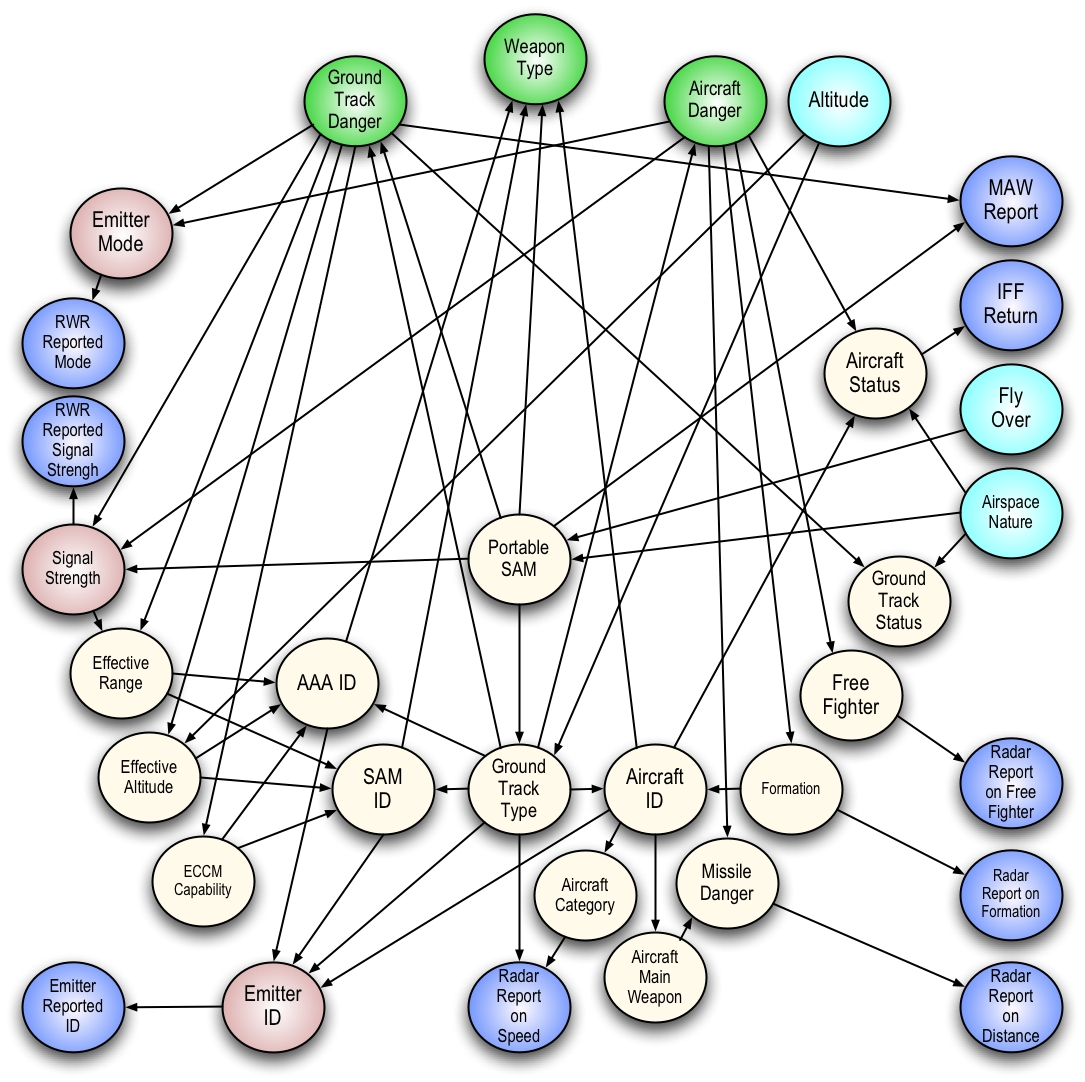
\includegraphics[scale=.25]{bn_wisepilot.jpg}
  \caption{Example of a Bayesian Network}
  \label{fig:bayes}
\end{figure}

Learning Bayesian networks automatically from data involves learning
the \emph{structure}, i.e., the conditional dependencies between the
random variables, and \emph{learning the parameters}, i.e., the
entries in the CPTs. Given a Bayesian network with a fixed structure,
it is possible to learn the parameters automatically from data.

\subsection{Bayesian Logic Programs}
Bayesian logic programs (BLPs) are templates for constructing directed
graphical models (Bayesian networks). BLP consists of a set of
Bayesian clauses, definite clauses of the form $a | a_1, a_2, a_3,
\ldots a_n$, where $n \geq 0$ and $a_1, a_2, a_3, \ldots a_n$ are
Bayesian predicates. $a$ is, $\mathtt{head}(c)$, the head of the
clause $c$, and $(a_1, a_2, a_3 \ldots a_n)$ is $\mathtt{body}(c)$,
the body. When $n = 0$, a Bayesian clause is a fact. Each Bayesian
clause $c$ is assumed to be universally quantified and range
restricted, i.e., $\{\mathtt{head}(c)\} \subseteq
\{\mathtt{body}(c)\}$, and has an associated conditional probability
table $\mathtt{CPT}(c) = P(\mathtt{head}(c)|\mathtt{body}(c))$. A
Bayesian predicate is a predicate with a finite domain, and each
ground atom for a Bayesian predicate represents a random variable.

\section{Literature survey}
Some of the existing approaches use Inductive Logic Programming that
do not use probabilistic graphical model to compute conditional
probabilities for inferred facts. To avoid this, a statistical
relational learning approach is adopted. SRL handles both uncertainty
and structured data, integrating first-order logic and probabilistic
graphical models. The alternative is to take SRL approaches such as
Markov Logic Networks (MLN) framework for both learning first order
rules and probabilistic inference of additional facts. But MLN may
result in an intractably large graphical model for large datasets.

To avoid this, another statistical relational learning approach,
namely BLP is adopted. Using Bayesian logic programs, directed
graphical models called Bayesian networks are constructed. Bayesian
networks are much smaller than the networks which are constructed by
MLN \cite{sindhu2012, sindhu2013}.

Learning commonsense knowledge in the form of first-order rules is
done by using the noisy extractions produced by an off-the-shelf IE
system. Those rules are then used to infer implicit information from
explicitly stated facts.

\begin{figure}[H]
  \centering
  % Define block styles

  \tikzstyle{i} = [rectangle, draw=none, text width=10em, text height
  = 18, text depth = 1cm, text centered, inner sep=0pt,minimum
  height=1em]

  \tikzstyle{o} = [rectangle, draw=none, text width=10em, text
  height = 15, text depth = 1cm, text centered, inner sep=0pt,minimum
  height=1em]

  \tikzstyle{block} = [rectangle, draw, text width=10em, text centered,
  minimum height=2em] \tikzstyle{line} = [draw, -latex']

  \tikzstyle{oval} = [rectangle, draw, text width=10em, text
  centered, rounded corners, minimum height=2em] \tikzstyle{line} =
  [draw, -latex']
    
  \begin{tikzpicture}[node distance = 2cm, auto]
    % Place nodes
    \node [oval](in) {Training data};
    \node [block, below of=in] (ie) {IE system};
    \node [oval, below of=ie] (facts) {Extracted facts};
    \node [block, below of=facts] (wtlearner) {BLP weight learner};
    \node [oval, below of=wtlearner] (fcount) {Frequency count of predicates};
    \node [block, below of=fcount] (infer) {BLP inference engine};
     \node [oval, below of=infer](out) {Inference rules};
    % Draw edges
    \path [line] (in) -- (ie);
    \path [line] (ie) -- (facts);
    \path [line] (facts) --  (wtlearner);
    \path [line] (facts.west) -- +(-0.5,0.0) |- (infer);   
    \path [line] (wtlearner) -- (fcount);
    \path [line] (fcount) --  (infer);
    \path [line] (infer) -- (out);
  \end{tikzpicture}
  \caption{System Architecture}
  \label{arch}
\end{figure}

\section{Proposed system}

A Rule Learner is applied on the set of facts an IE system has
extracted from the document. The Rule Learner first updates the
frequency of occurrence of each relational predicate. Then it builds a
Bayesian network whose nodes represent relation extractions. It then
traverses the graph to know the first order rules. The learner
traverses the resulting graph to construct rules. For each directed
edge $(x,y)$ in the graph, it constructs a rule in which the body
contains $x$ and the head is $y$ head. System architecture for
inferring implicit facts using BLPs is shown in Figure~\ref{arch}.


\begin{thebibliography}{99}
  \bibliographystyle{plain}
  
\bibitem[1]{sindhu2013} Sindhu Raghavan, Raymond J. Mooney, {\em
    Online Inference-Rule Learning from Natural-Language Extractions},
  University of Texas at Austin, In Proceedings of the 3rd Statistical
  Relational AI (StaRAI-13) workshop at AAAI '13, July 2013.

\bibitem[2]{sindhu2012}Sindhu Raghavan, Raymond J. Mooney, and
  Ku. H,{\em to read between the lines using Bayesian Logic Programs},
  In Proceedings of ACL 2012.

\bibitem[3]{cowir1996}Cowie, J., and Lehnert, W. ,{\em Information
    extraction}, 1996 CACM.

\bibitem[4]{kersting2007}Kersting, K., and De Raedt, L., {\em Bayesian
    Logic Programming: Theory and tool}, 2007

\bibitem[5]{5} In Getoor, L., and Taskar, B, {\em Introduction to
    Statistical Relational Learning}, Cambridge, MA: MIT Press.
\end{thebibliography}


	
\end{document}
